%% LyX 2.0.5.1 created this file.  For more info, see http://www.lyx.org/.
%% Do not edit unless you really know what you are doing.
\documentclass[english,compress,serif]{beamer}
\usepackage{mathptmx}
\usepackage[T1]{fontenc}
\usepackage[latin9]{inputenc}
\usepackage{array}
\usepackage{multirow}
\usepackage{amsmath}
\usepackage{amssymb}
\usepackage{graphicx}
\usepackage[numbers]{natbib}

\makeatletter

%%%%%%%%%%%%%%%%%%%%%%%%%%%%%% LyX specific LaTeX commands.
\newcommand{\noun}[1]{\textsc{#1}}
%% Because html converters don't know tabularnewline
\providecommand{\tabularnewline}{\\}
%% A simple dot to overcome graphicx limitations
\newcommand{\lyxdot}{.}


%%%%%%%%%%%%%%%%%%%%%%%%%%%%%% Textclass specific LaTeX commands.
 % this default might be overridden by plain title style
 \newcommand\makebeamertitle{\frame{\maketitle}}%
 \AtBeginDocument{
   \let\origtableofcontents=\tableofcontents
   \def\tableofcontents{\@ifnextchar[{\origtableofcontents}{\gobbletableofcontents}}
   \def\gobbletableofcontents#1{\origtableofcontents}
 }
 \long\def\lyxframe#1{\@lyxframe#1\@lyxframestop}%
 \def\@lyxframe{\@ifnextchar<{\@@lyxframe}{\@@lyxframe<*>}}%
 \def\@@lyxframe<#1>{\@ifnextchar[{\@@@lyxframe<#1>}{\@@@lyxframe<#1>[]}}
 \def\@@@lyxframe<#1>[{\@ifnextchar<{\@@@@@lyxframe<#1>[}{\@@@@lyxframe<#1>[<*>][}}
 \def\@@@@@lyxframe<#1>[#2]{\@ifnextchar[{\@@@@lyxframe<#1>[#2]}{\@@@@lyxframe<#1>[#2][]}}
 \long\def\@@@@lyxframe<#1>[#2][#3]#4\@lyxframestop#5\lyxframeend{%
   \frame<#1>[#2][#3]{\frametitle{#4}#5}}
 \def\lyxframeend{} % In case there is a superfluous frame end

%%%%%%%%%%%%%%%%%%%%%%%%%%%%%% User specified LaTeX commands.
\usepackage{color}
\definecolor{RiceBlue}{cmyk}{1,0.93,0.28,0.22}
\definecolor{RiceGray}{cmyk}{0,0,0,0.77}
\usetheme{Singapore} 
\usecolortheme[named=RiceGray]{structure}
%\usetheme{Luebeck}
%\usecolortheme{beaver}
\usepackage{textpos}

\setbeamercolor{titlelike}{fg=RiceBlue}

\setbeamercovered{transparent}
% or whatever (possibly just delete it)

%\pgfdeclareimage[height=1cm]{institution-logo}{RiceLogo_TMCMYK300DPI.jpg}
%\logo{\includegraphics[height=7mm]{RiceLogo_TMCMYK300DPI.jpg}\vspace{220pt}}
%\logo{\includegraphics[height=1cm]{RiceLogo_TMCMYK300DPI.jpg}}
\addtobeamertemplate{frametitle}{}{%
\begin{textblock*}{100mm}(-.93cm,7.57cm)
\includegraphics[height=.75cm]{figures/RiceLogo_TMCMYK300DPI.jpg}
%\includegraphics[height=.4cm]{RUTypeTM(Blue)CMYK300DPI.jpg}
%\tiny Department of Electrical Engineering - Rice University - April 18, 2013
\end{textblock*}}

\setbeamertemplate{caption}[numbered]

\makeatother

\usepackage{babel}
\begin{document}

\title{Using Artificial Neural Networks in the \emph{stop squark }Search}


\author{R. Brockman, J.~DeVito, and R. LeVan}


\institute{Department of Electrical Engineering\\
Rice University }


\date{Spring 2013\\
\vspace{0.12\paperheight}
\includegraphics[height=1.25cm]{figures/RiceLogo_TMCMYK300DPI}
\qquad \qquad
\includegraphics[height=1.25cm]{figures/ECE_Logo}}

\makebeamertitle


%\AtBeginSubsection[]{
%  \frame<beamer>{ 
%    \frametitle{Outline}   
%    \tableofcontents[currentsection,currentsubsection] 
%  }
%}
%
%If you wish to uncover everything in a step-wise fashion, uncomment the following command:
%\beamerdefaultoverlayspecification{<+->}


\lyxframeend{}\lyxframe{Outline}

\tableofcontents{}


\lyxframeend{}\section{Background}


\lyxframeend{}\subsection{Introduction}


\lyxframeend{}\lyxframe{Introduction}
\begin{block}
{Overall Plan}

From a large data set we try to separate a signal from a specific
type of noise.\end{block}
\begin{itemize}
\item Signal $:=$ \emph{stop squark }event
\item Noise $:=$ top quark background event
\item Use SOM and Back-prop as filters
\end{itemize}

\lyxframeend{}\lyxframe{Purpose}
\begin{itemize}
\item Search for the \emph{stop squark}, predicted by SUSY
\item Guided by Dr. Paul Padley of Bonner Lab 
\item Simulated data generated by PYTHIA
\end{itemize}

\begin{block}
{Aim}

Improve on the results in the paper by Dutta, et al. \citep{:Dutta2012},
working in parallel with Onkur Sen, who is attacking the same problem
using boosted decision trees. 
\end{block}

\lyxframeend{}\lyxframe{What is a \emph{stop squark} Event?}

\begin{center}
\includegraphics{figures/Schematic_Signal_Noise}{\tiny \citep{:Dutta2012}}
\par\end{center}


\lyxframeend{}\section{Methods}


\lyxframeend{}\subsection{Classification Basics}


\lyxframeend{}\lyxframe{Classification Basics}

From the simulated data, with the help of Onkur's code, we were able
to create:
\begin{itemize}
\item a length 24 vector of raw data for each signal or background event

\end{itemize}

\begin{itemize}
\item a length 8 vector of derived variables from the raw data \citep{:Dutta2012}
\end{itemize}
Previously attempted strategy:
\begin{itemize}
\item Thresholds on derived variables as outlined in Dutta, et al. \citep{:Dutta2012} 
\end{itemize}

\lyxframeend{}\subsection{Significance}


\lyxframeend{}\lyxframe{Significance: A Filter Comparison Metric}
\begin{itemize}
\item A measure of discovery confidence based on a certain number of high
energy particle collisions
\end{itemize}
\[
\mbox{significance}=\frac{N_{\mbox{Signal}}}{\sqrt{N_{\mbox{Background}}}}
\]


$N_{\mbox{Signal}}:=$ number of signal events that come through the
filter

$N_{\mbox{Background}}:=$ number of noise events that come through
the filter
\begin{itemize}
\item Used commonly in physics 
\item Every significance measure in the Results Section is based on a standard
number of collisions
\end{itemize}

\lyxframeend{}\subsection{Neural Network Filters}


\lyxframeend{}\lyxframe{Back-Propagation Filter Settings}

\noindent \begin{center}
\qquad{}{\small%
\begin{tabular}{cc}
\hline 
\multicolumn{2}{c}{\textbf{\noun{\large Architecture}}}\tabularnewline
\hline 
Topology & (8 +$1_{Bias}$) - (30 +$1_{Bias}$) - 2$_{output}$ \tabularnewline
Transfer Function & $\tanh$ with slope $b=1$\tabularnewline
\hline 
\multicolumn{2}{c}{\textbf{\noun{\large Learning Parameters}}}\tabularnewline
\hline 
Initial weights & $w\sim U[-0.1,\,0.1]$\tabularnewline
Learning rate, $\gamma(t)$ & $\gamma(t)=0.01(1-0.0001)^{t}$\tabularnewline
Momentum, $\alpha$ & $\alpha=0.3$\tabularnewline
Epoch size & $K=1$\tabularnewline
Stopping criteria & learning step > 100,000\tabularnewline
Error measure (Err) & RMSE \tabularnewline
Monitoring frequency (m) & 1,000 Learning Steps\tabularnewline
\hline 
\multicolumn{2}{c}{\textbf{\noun{\large Input/Output Scaling}}}\tabularnewline
\hline 
Input Scaling & (-0.9,0.9)\tabularnewline
Output Scaling & (-0.9,0.9)\tabularnewline
\hline 
\multicolumn{2}{c}{\textbf{\noun{\large Performance Evaluation}}}\tabularnewline
\hline 
Accuracy measure ($\mbox{Acc}_{X}$) & Significance = $\frac{S}{\sqrt{B}}$\tabularnewline
\hline 
 & \tabularnewline
\end{tabular}}\qquad{}
\par\end{center}


\lyxframeend{}\lyxframe{Self-Organizing Map Filter Settings}

\noindent \begin{center}
\qquad{}{\small%
\begin{tabular}{cc}
\hline 
\multicolumn{2}{c}{\textbf{\noun{\large Architecture}}}\tabularnewline
\hline 
Topology & 10 x 10\tabularnewline
\hline 
\multicolumn{2}{c}{\textbf{\noun{\large Learning Parameters}}}\tabularnewline
\hline 
Initial weights & $w\sim U[-0.1,\,0.1]$\tabularnewline
Learning rate, $\gamma(t)$ & $\gamma(t)=0.3(1-0.00001)^{t}$\tabularnewline
Neighborhood, $\sigma(t)$ & $\sigma(t)=1.5+3.5\left(1-0.00001\right)^{t}$\tabularnewline
Epoch size & $K=1$\tabularnewline
Stopping criteria & learning step > 750,000\tabularnewline
Monitoring frequency (m) & 1,000 Learning Steps\tabularnewline
\hline 
\multicolumn{2}{c}{\textbf{\noun{\large Input/Output Scaling}}}\tabularnewline
\hline 
Input Scaling & Angles in Degrees, Otherwise None\tabularnewline
Output Scaling & None\tabularnewline
\hline 
\multicolumn{2}{c}{\textbf{\noun{\large Performance Evaluation}}}\tabularnewline
\hline 
Accuracy measure ($\mbox{Acc}_{X}$) & Significance = $\frac{S}{\sqrt{B}}$\tabularnewline
\hline 
 & \tabularnewline
\end{tabular}}\qquad{}
\par\end{center}


\lyxframeend{}\section{Results}


\lyxframeend{}\subsection{Back-Propagation Results}


\lyxframeend{}\lyxframe{Back-Propagation Results for Derived Variables}

\begin{center}
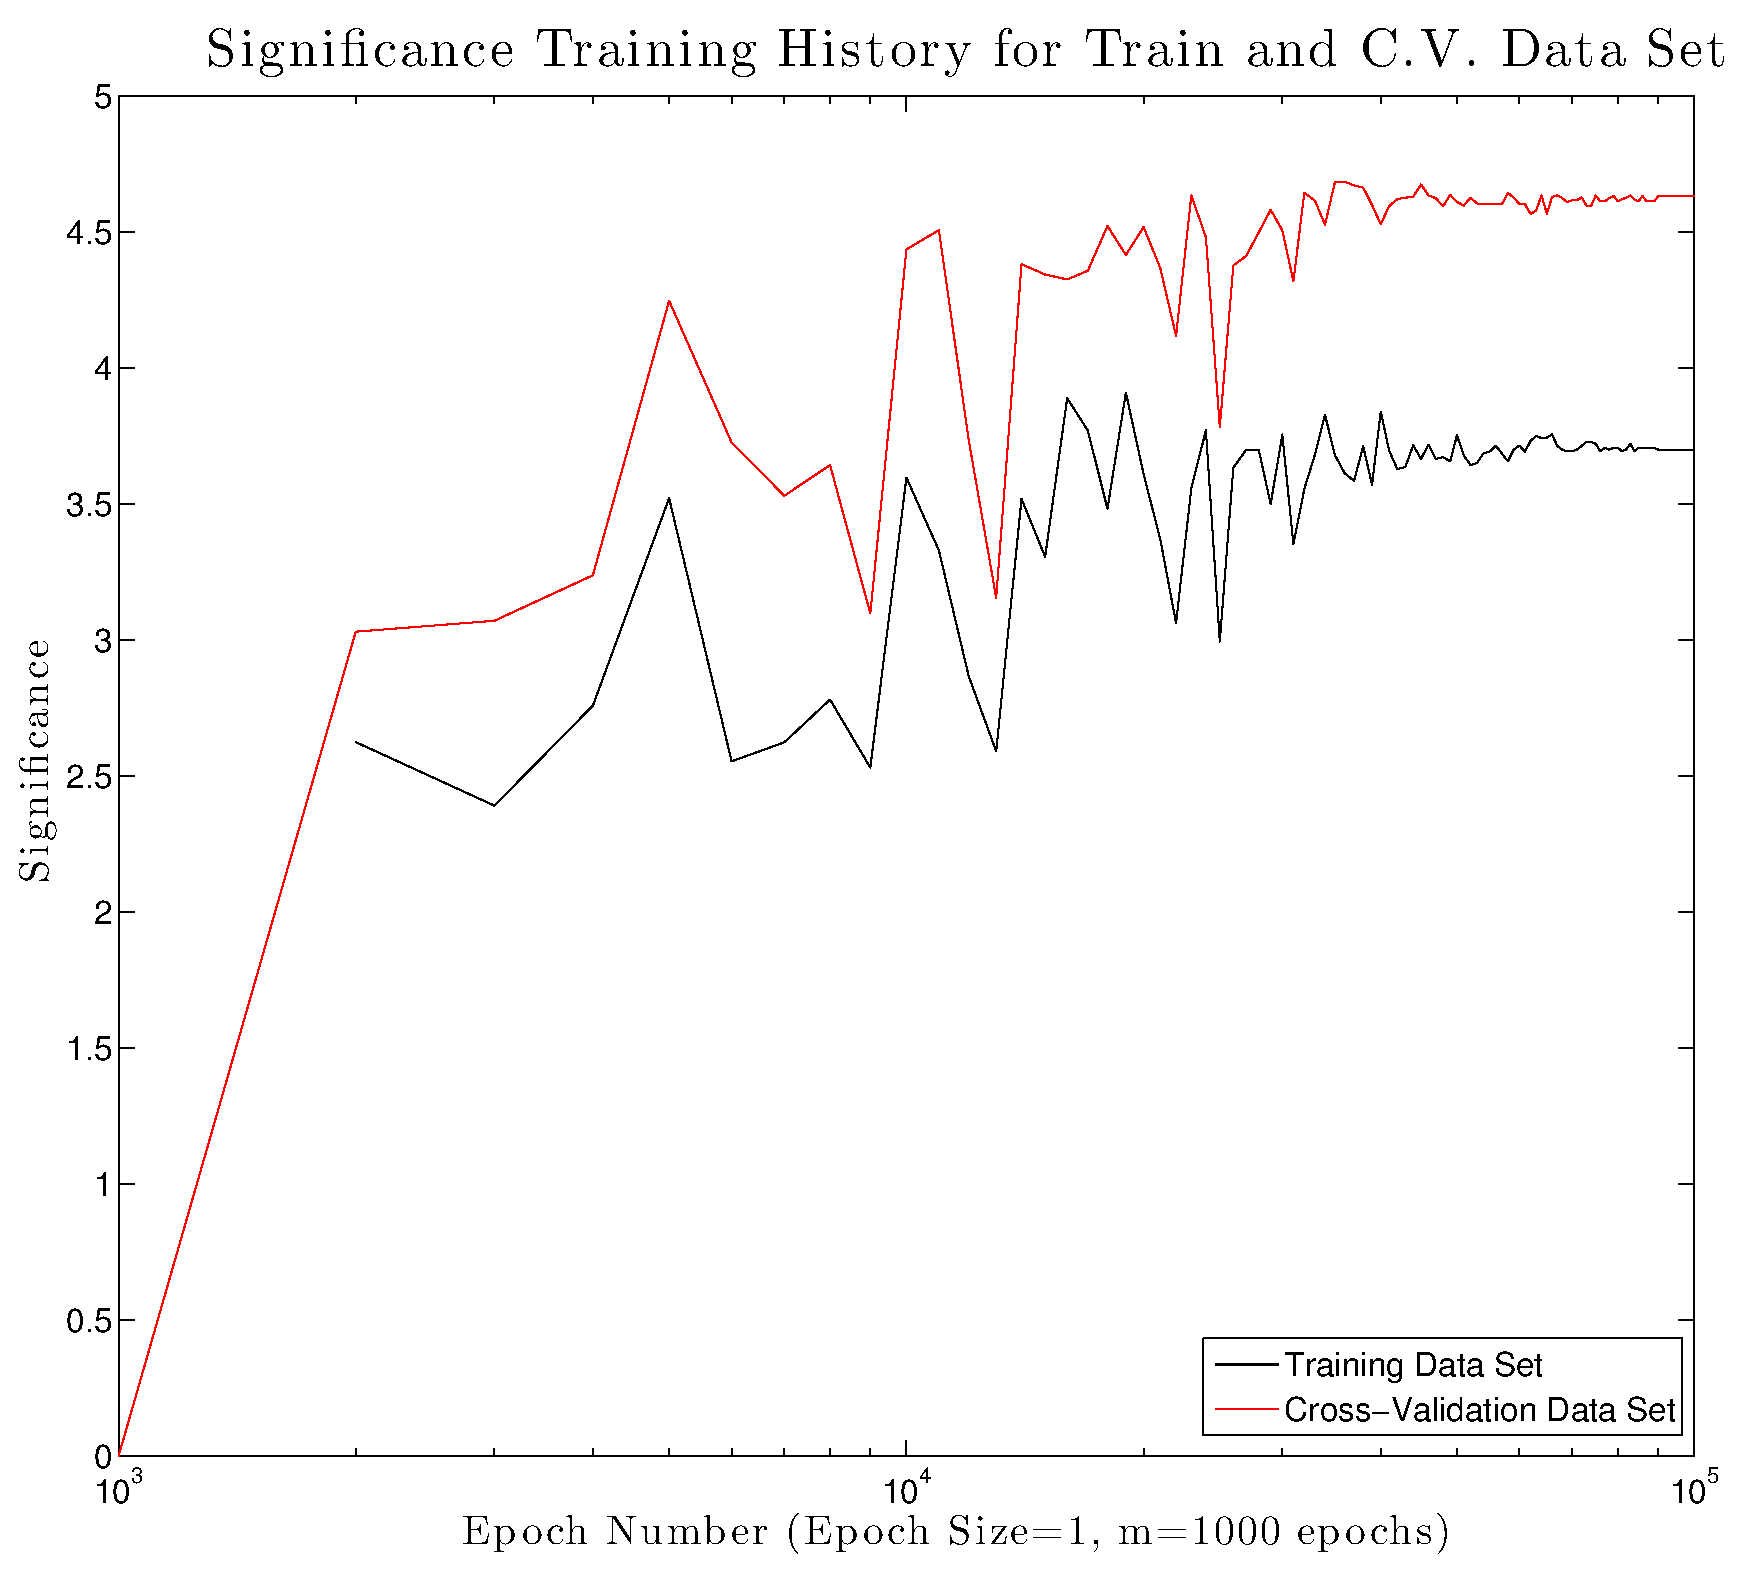
\includegraphics[height=0.75\paperheight]{/Users/me/Documents/Tower_Repository/comp502-physics/RobertBPcode/SigTrainHist_BP}
\par\end{center}


\lyxframeend{}\subsection{Self-Organizing Map Results}


\lyxframeend{}\lyxframe{SOM for Derived Variables}

\begin{center}
SOM Signal and Noise Density plots with weights 
\par\end{center}

\begin{center}
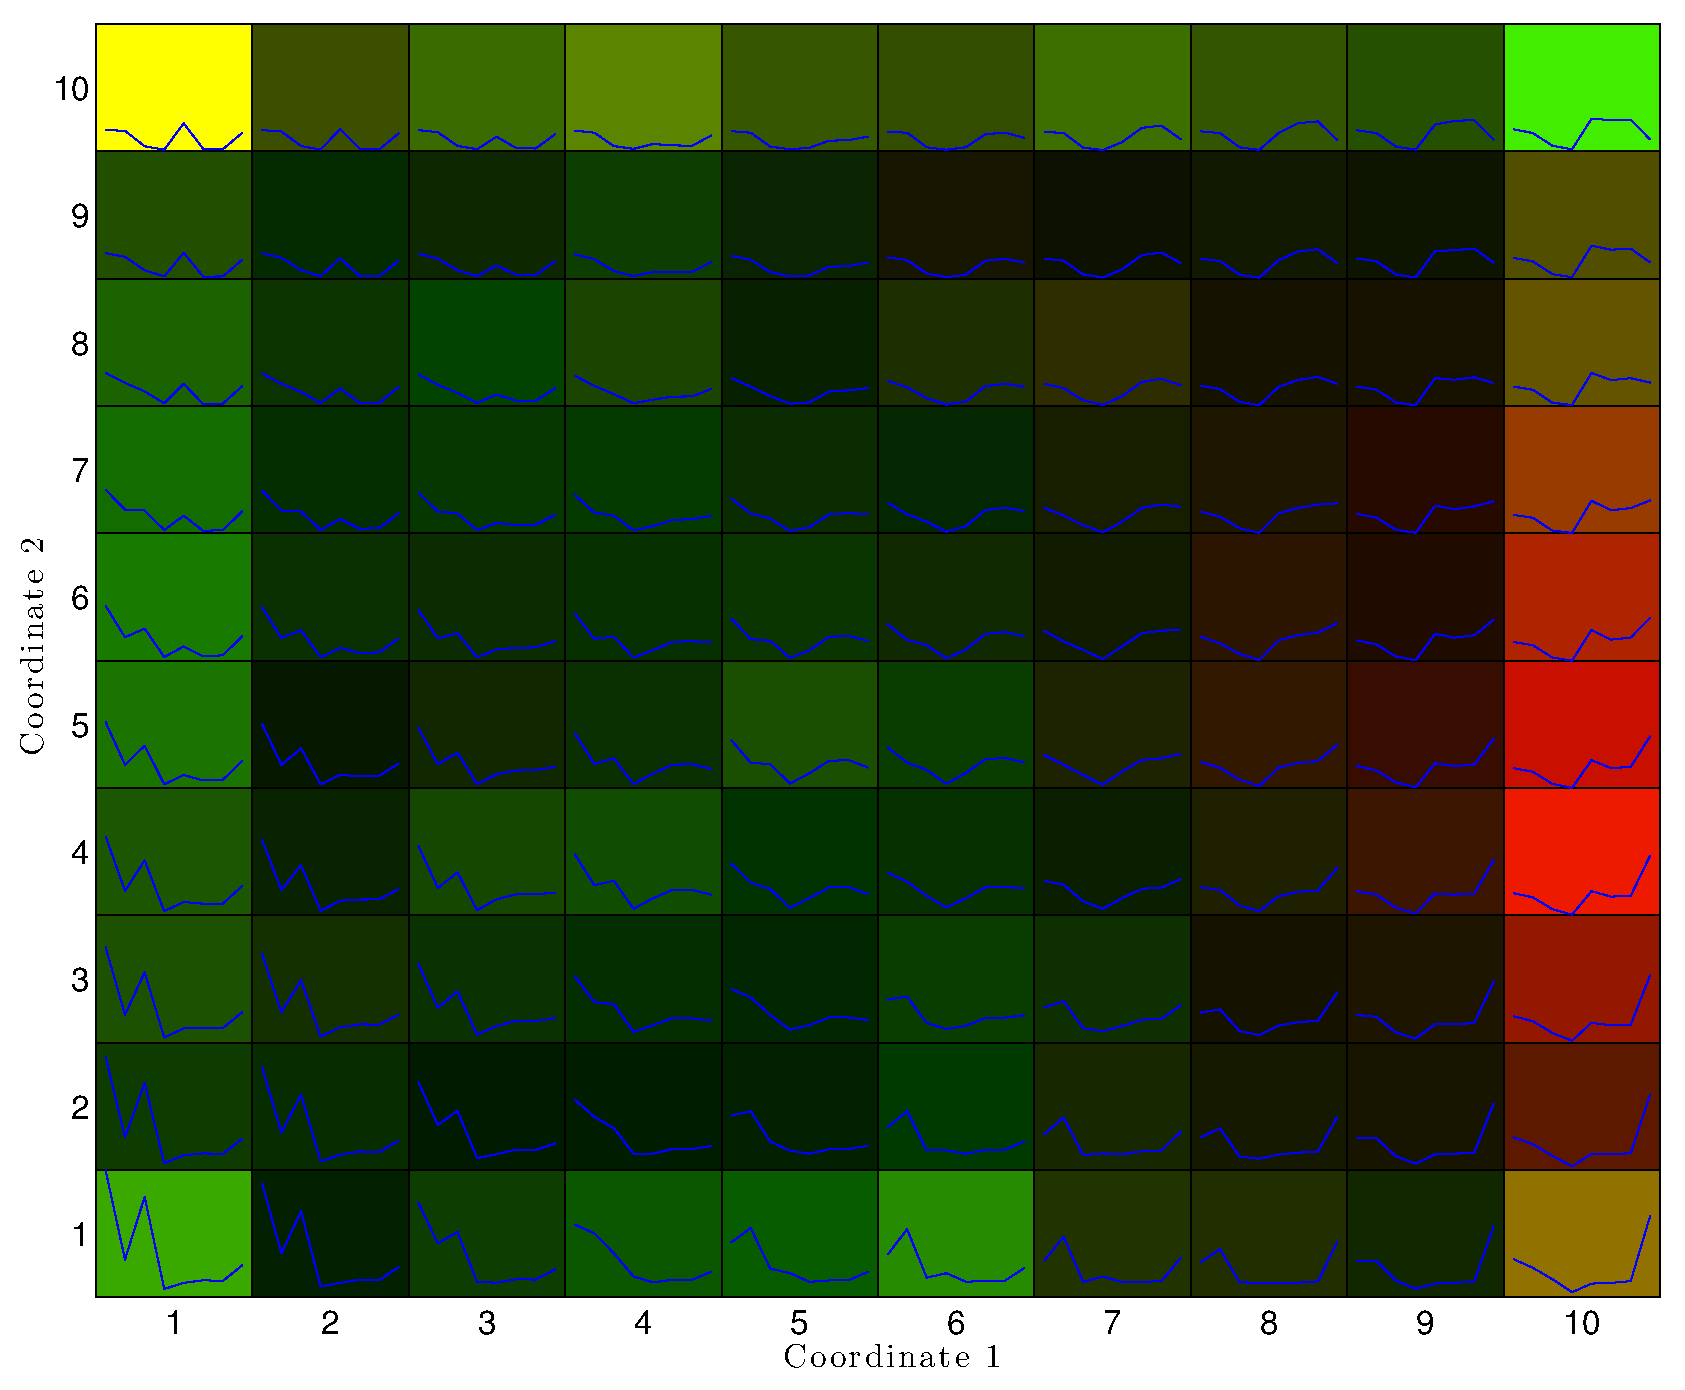
\includegraphics[height=0.6\paperheight]{\lyxdot \lyxdot /\lyxdot \lyxdot /RobertSOMcode/PrototypesGraph_8}\includegraphics[width=0.2\paperwidth]{figures/RGLegend}
\par\end{center}


\lyxframeend{}\lyxframe{SOM for Derived Variables}

\begin{center}
SOM Normalized Signal to Noise Ratios 
\par\end{center}

\begin{center}
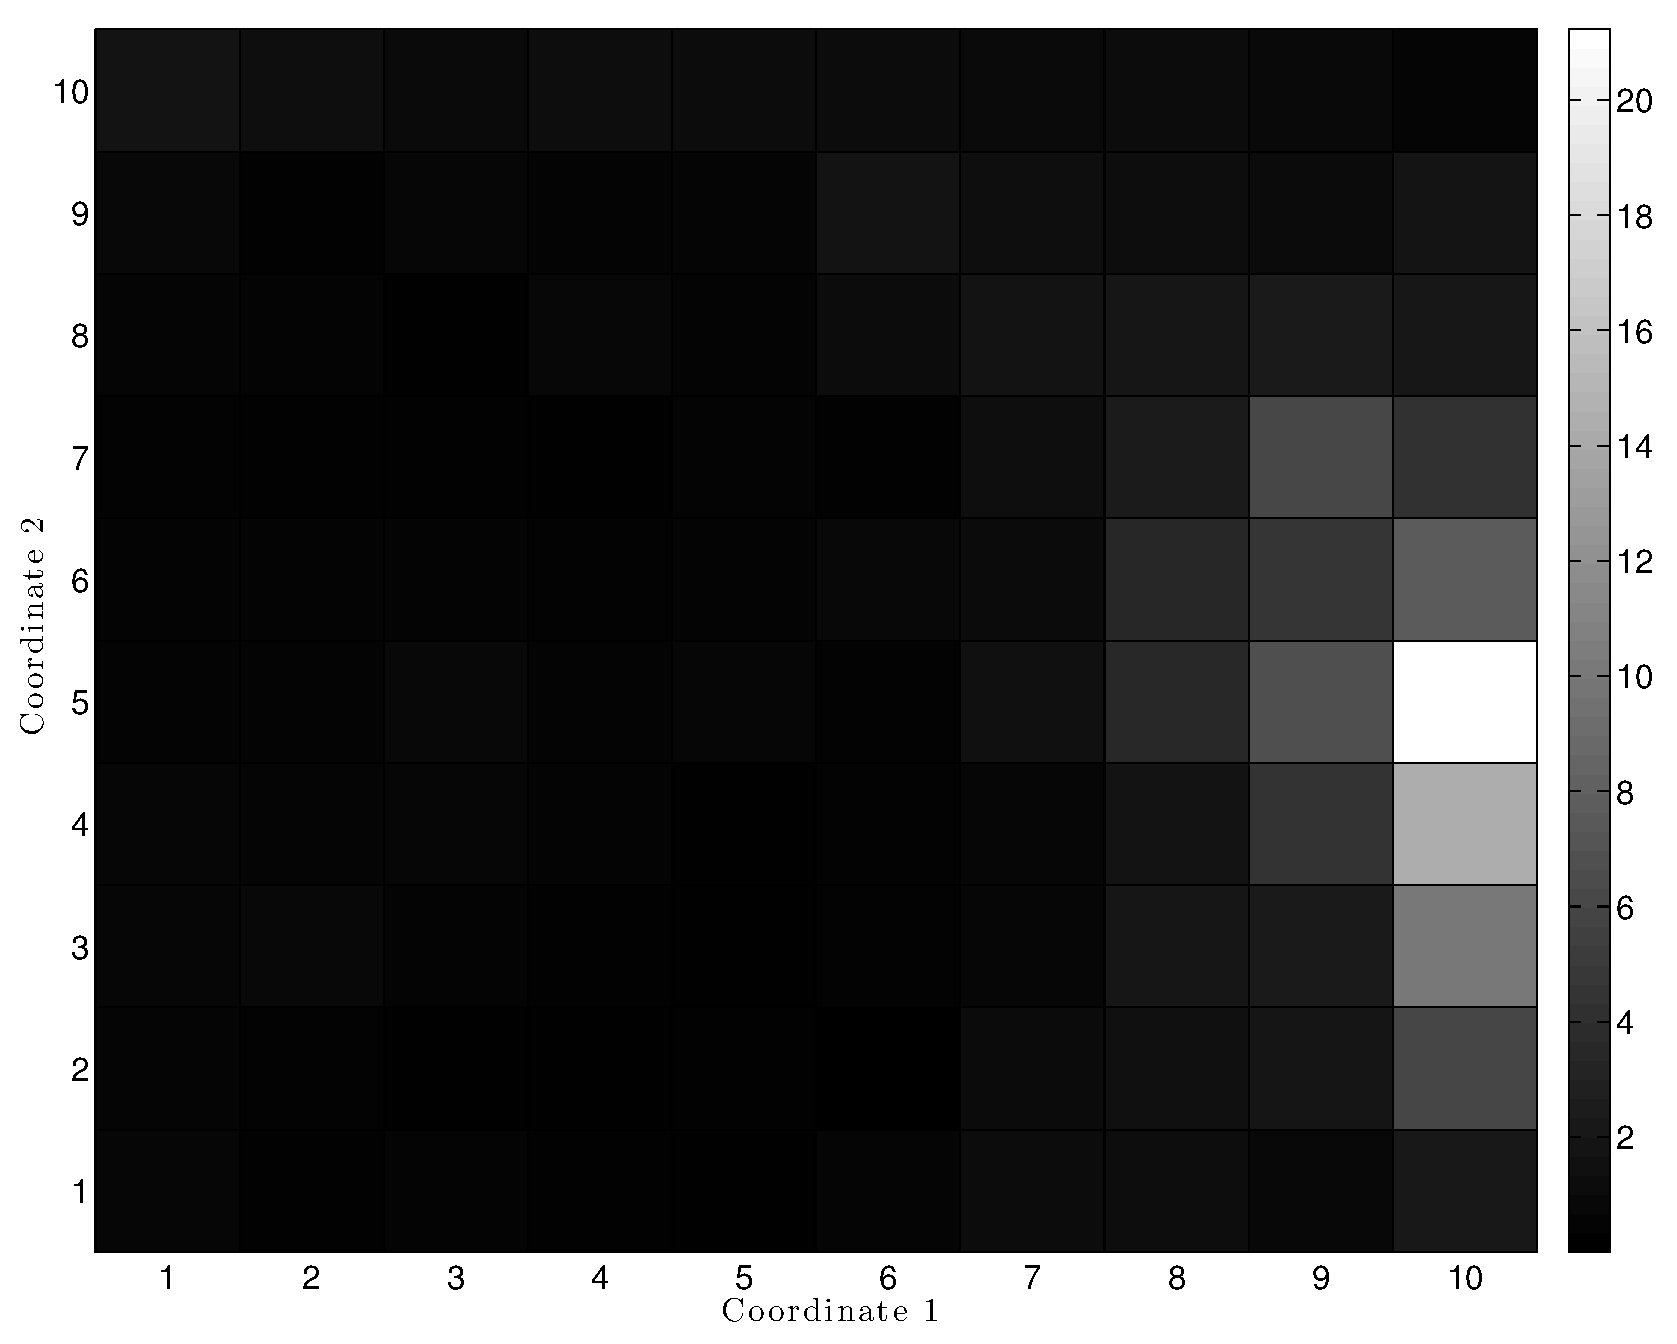
\includegraphics[height=0.7\paperheight]{\lyxdot \lyxdot /\lyxdot \lyxdot /RobertSOMcode/GainGraph_8}
\par\end{center}


\lyxframeend{}\lyxframe{SOM followed by BP for Derived Variables}

\begin{center}
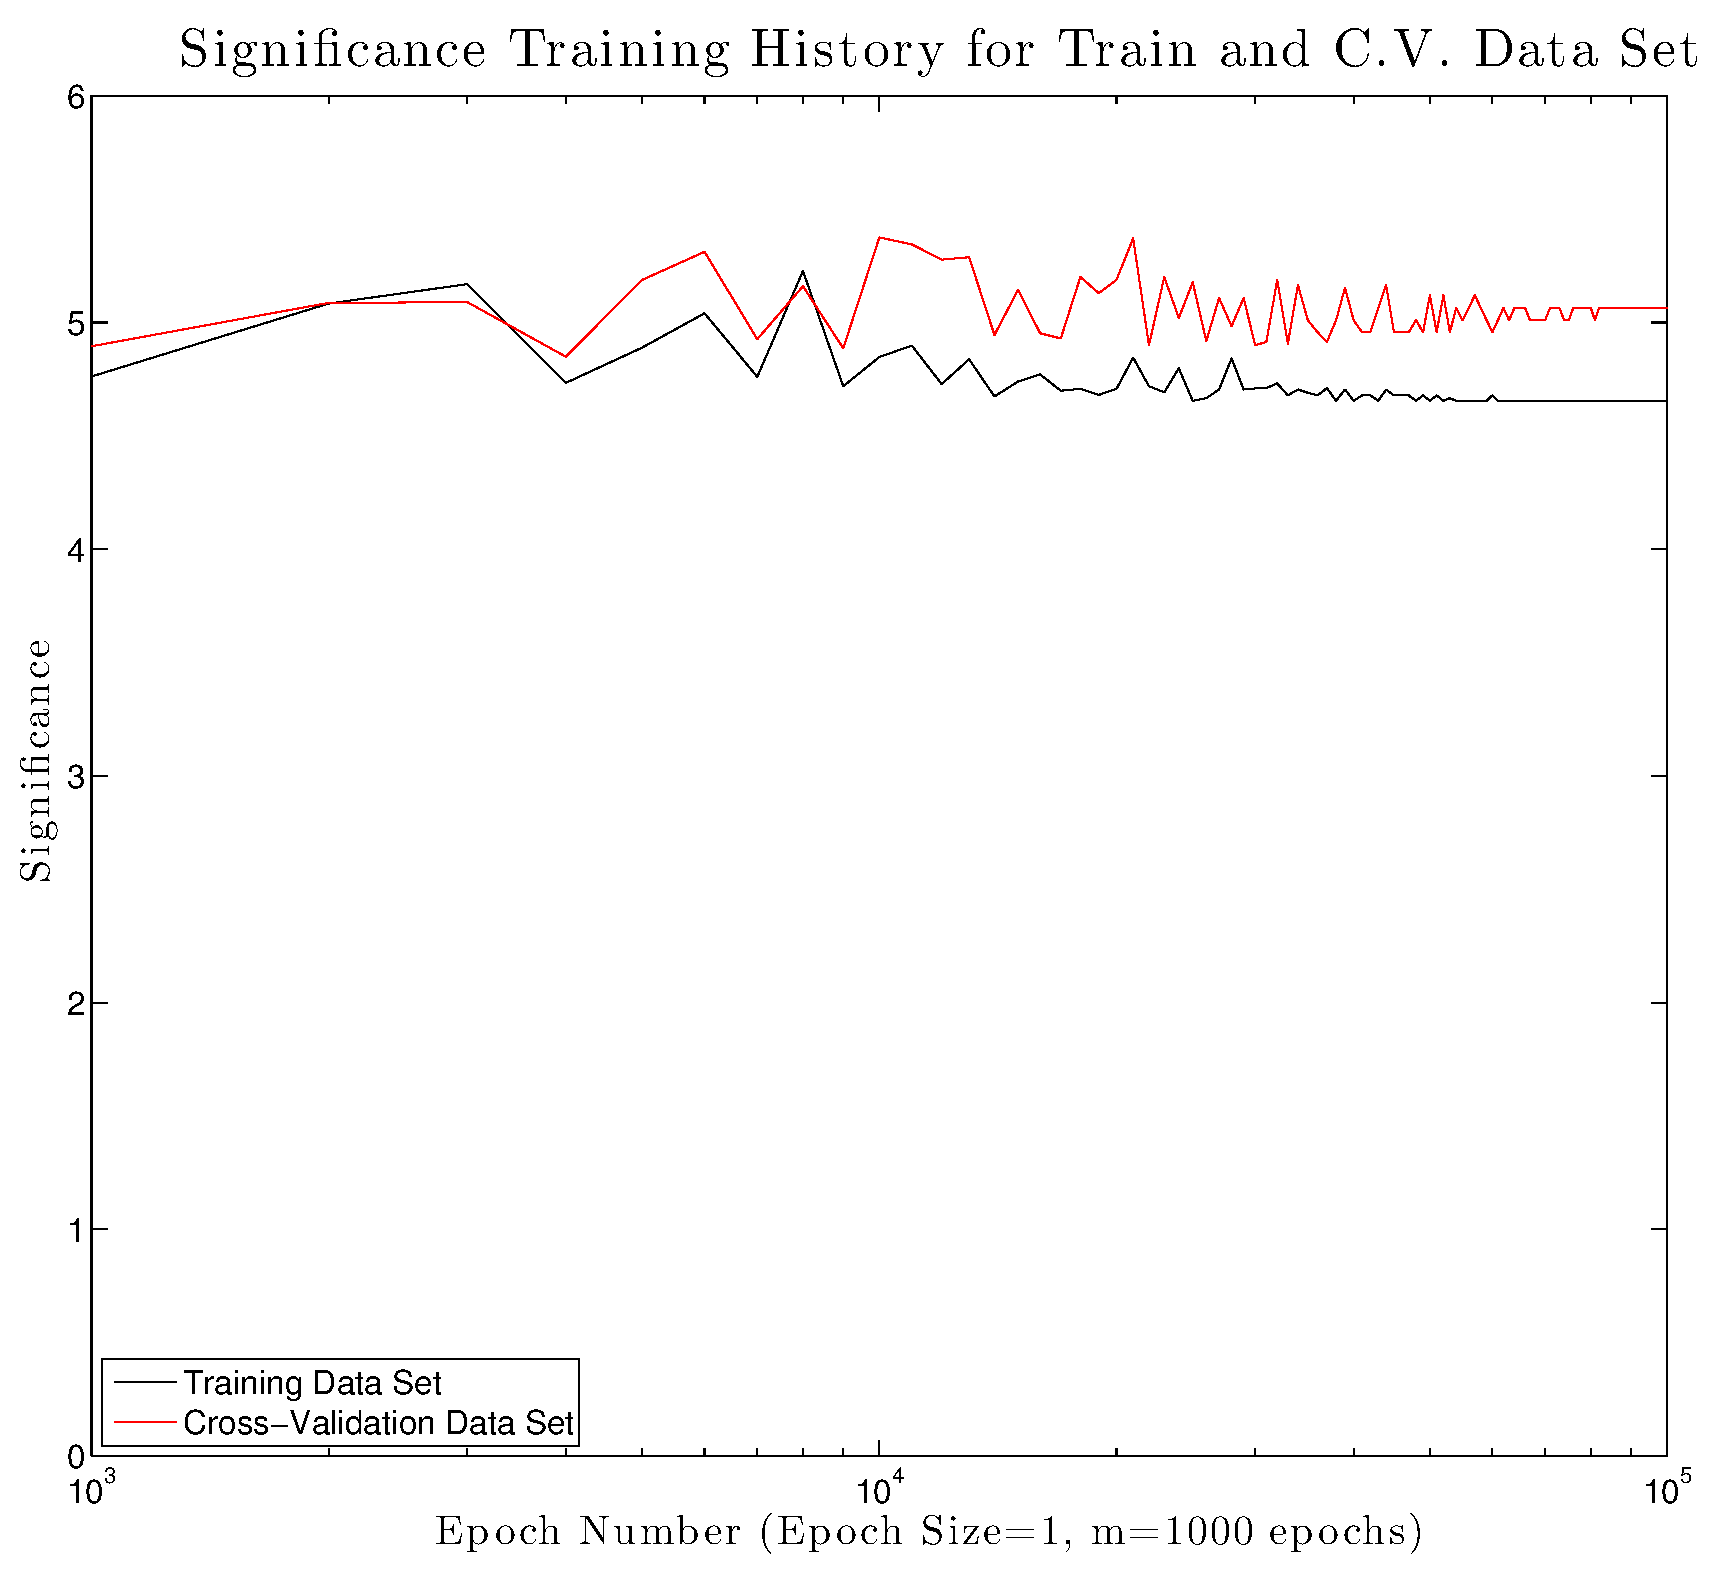
\includegraphics[height=0.75\paperheight]{\lyxdot \lyxdot /\lyxdot \lyxdot /RobertBPcode/SigTrainHist_BP_SOM_8}
\par\end{center}


\lyxframeend{}\lyxframe{SOM on Raw Data}

\begin{center}
SOM Signal and Noise Density plots with weights 
\par\end{center}

\begin{center}
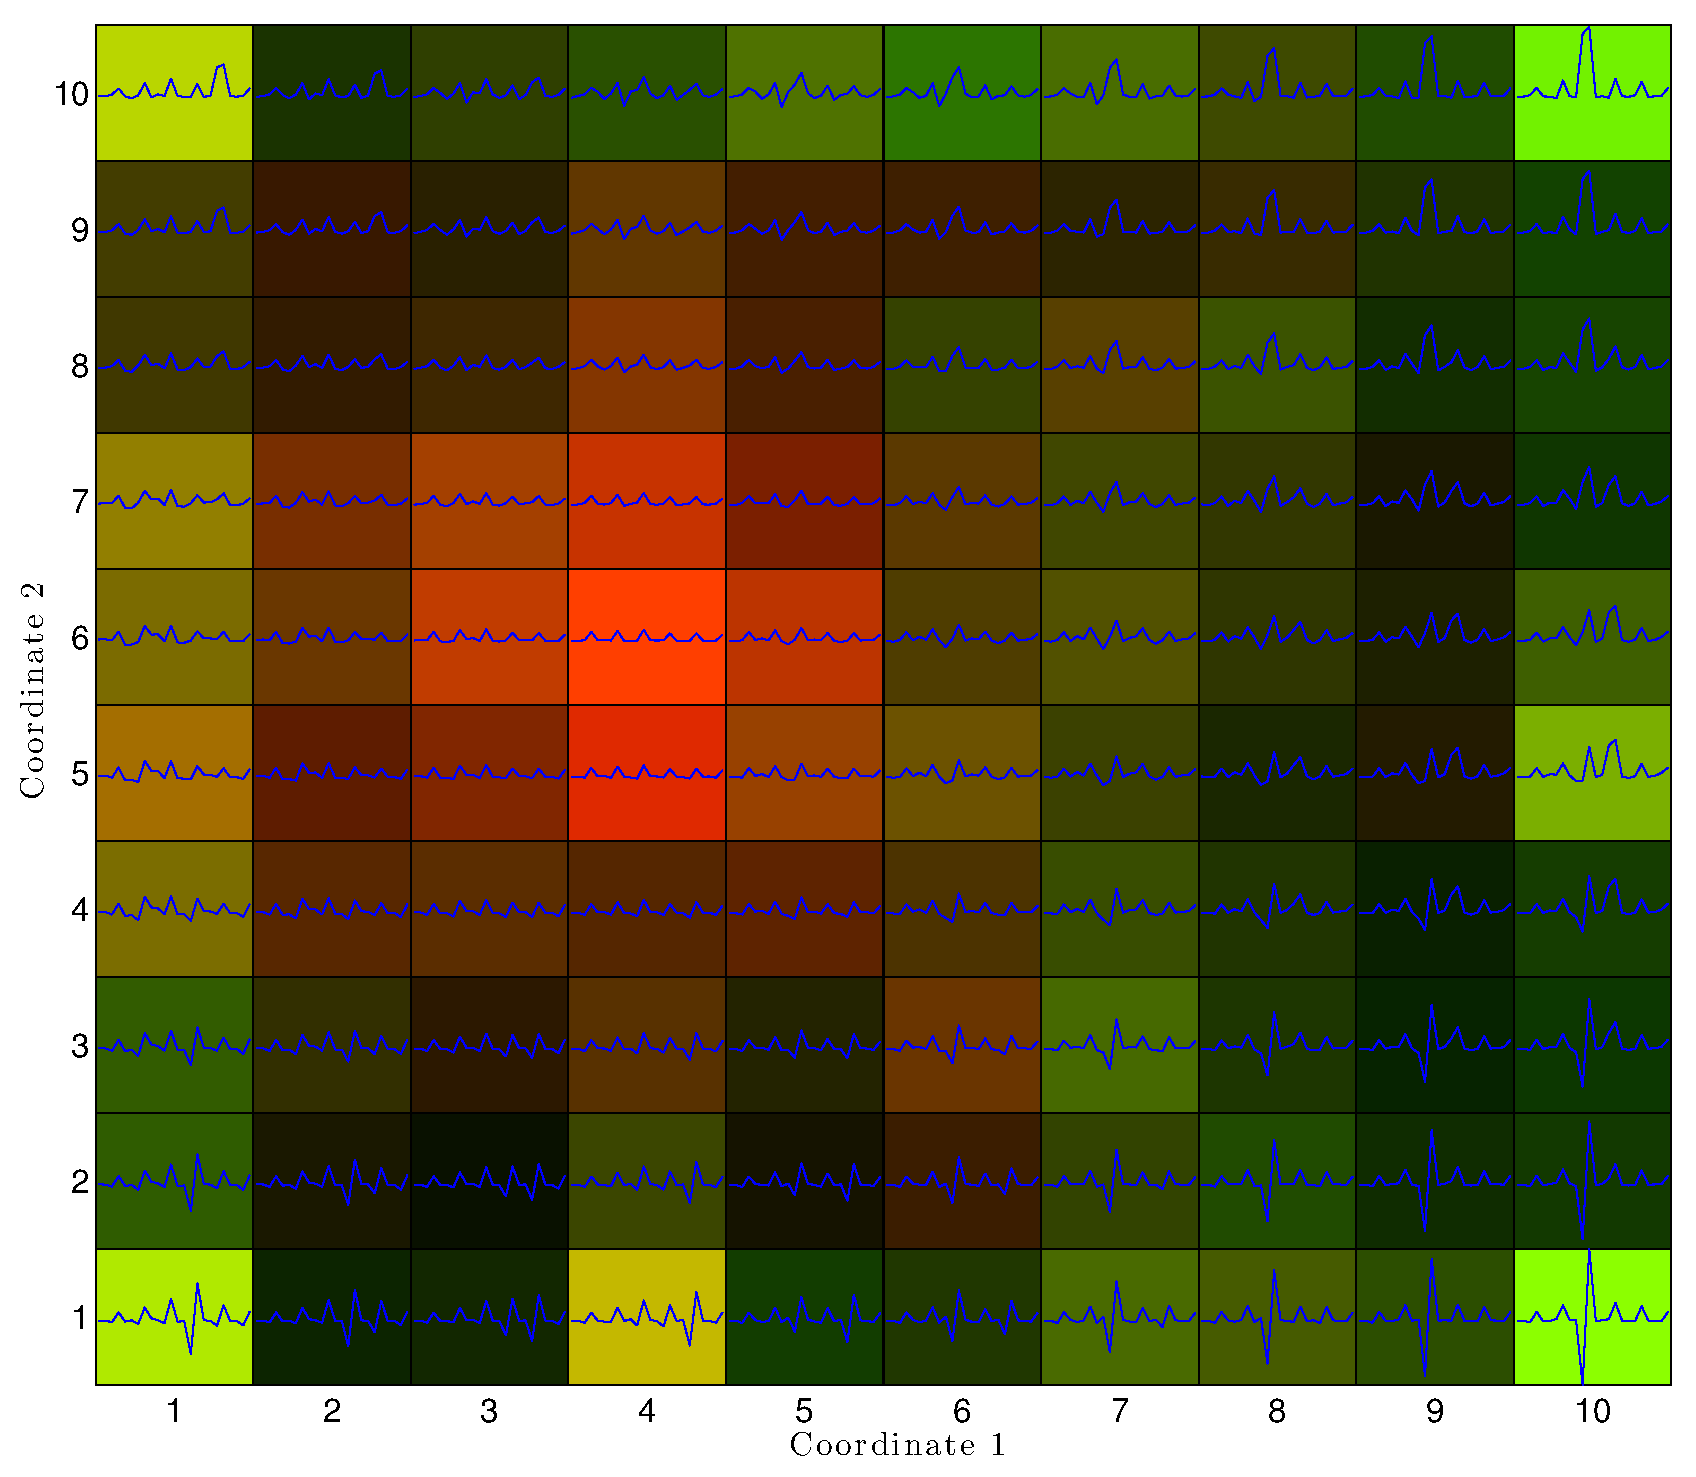
\includegraphics[height=0.6\paperheight]{\lyxdot \lyxdot /\lyxdot \lyxdot /RobertSOMcode/exemplarSquaresPlot_24}\includegraphics[width=0.2\paperwidth]{figures/RGLegend}
\par\end{center}


\lyxframeend{}\lyxframe{SOM on Raw Data}

\begin{center}
SOM Normalized Signal to Noise Ratios 
\par\end{center}

\begin{center}
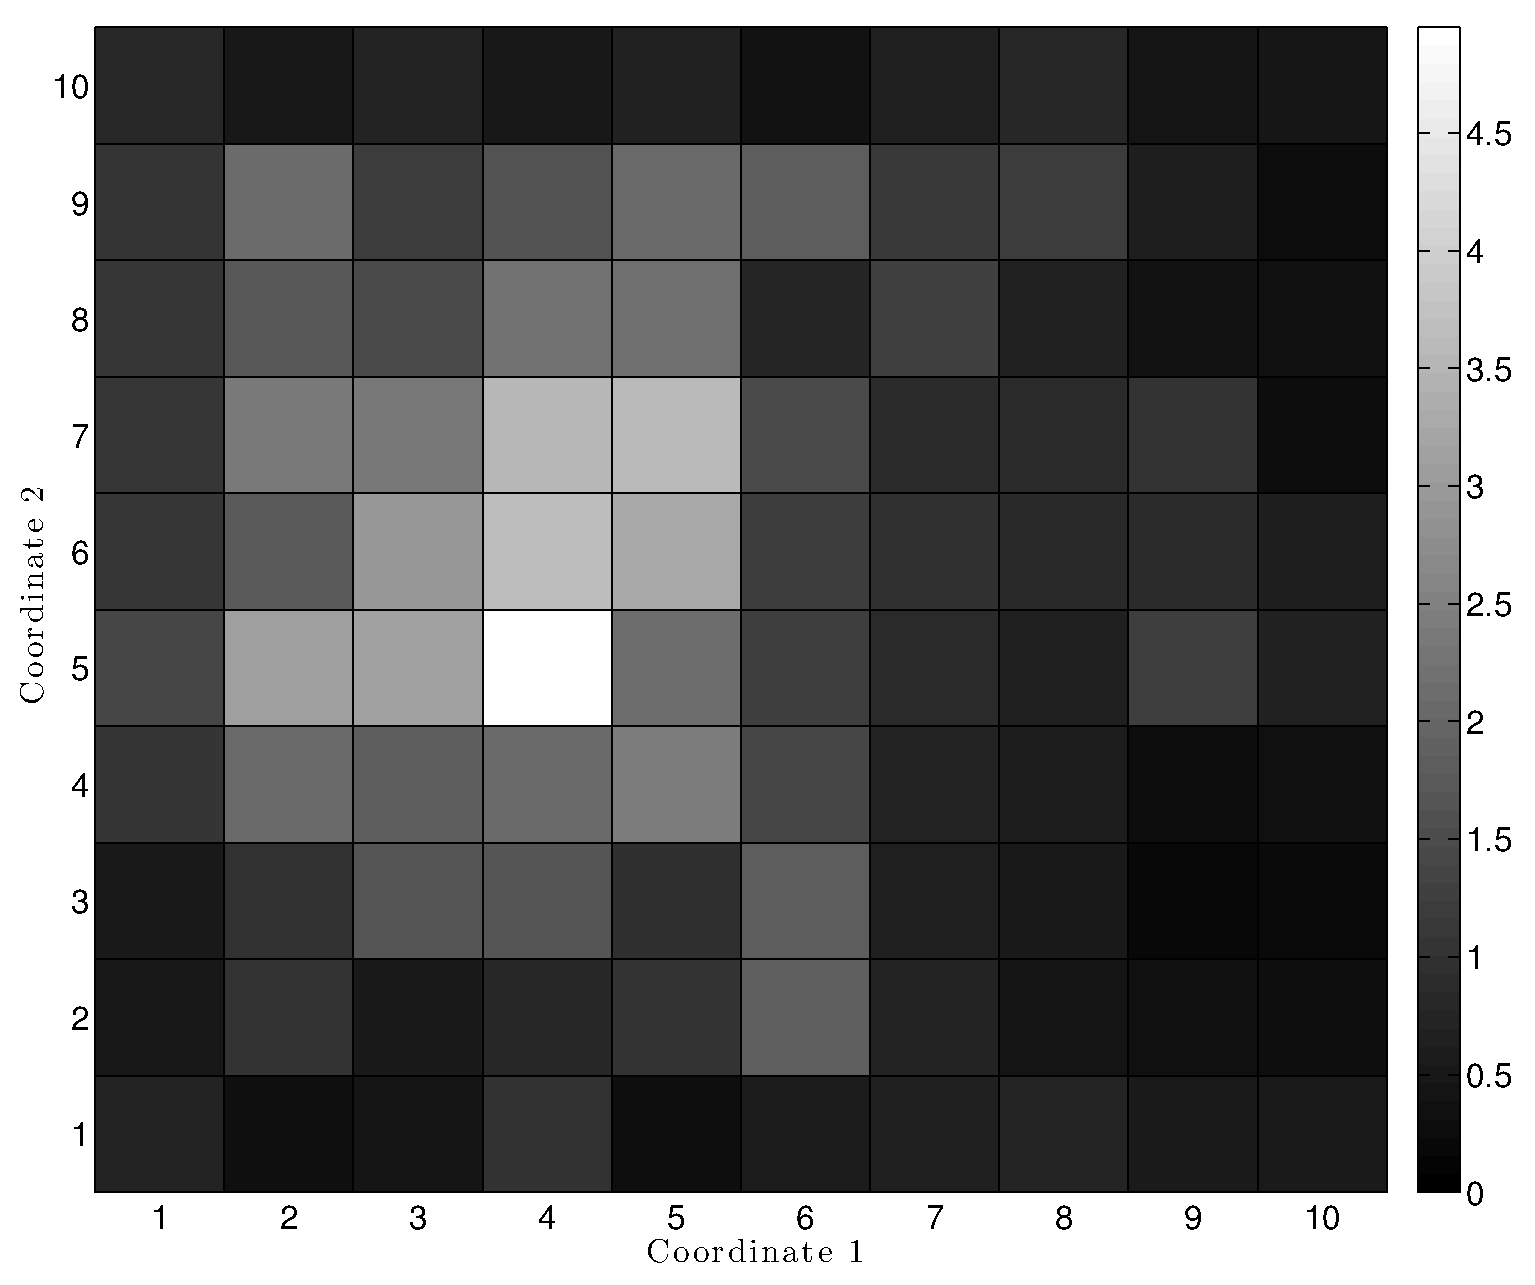
\includegraphics[height=0.7\paperheight]{\lyxdot \lyxdot /\lyxdot \lyxdot /RobertSOMcode/gain_24}
\par\end{center}


\lyxframeend{}\subsection{Analysis}


\lyxframeend{}\lyxframe{Significance Analysis}

\begin{center}
\begin{tabular}{|c|c|}
\hline 
\multirow{2}{*}{\textrm{\textbf{\textsc{\large Method}}}} & \textrm{\textbf{\textsc{\large Test Set}}}\tabularnewline
 & \textrm{\textbf{\textsc{\large Significance}}}\tabularnewline
\hline 
\textrm{\textcolor{blue}{\large Thresholding \citep{:Dutta2012}}} & \textrm{\textcolor{blue}{\large 1.93$\sigma$}}\tabularnewline
\hline 
\textrm{No Filter} & 2.62$\sigma$\tabularnewline
\hline 
\textrm{Back-Propagation} & 3.79$\sigma$\tabularnewline
\hline 
\textrm{Self-Organizing Map for Derived Variables} & 3.69$\sigma$\tabularnewline
\hline 
\textrm{\textcolor{red}{\large SOM then Back-Propagation}} & \textrm{\textcolor{red}{\large 4.36$\sigma$}}\tabularnewline
\hline 
\textrm{Self-Organizing Map for Raw Data} & 2.62$\sigma$\tabularnewline
\hline 
\end{tabular}
\par\end{center}


\lyxframeend{}\lyxframe{Analysis}
\begin{itemize}
\item Back-Propagation and the SOM using the 8 derived variables produced
interesting results
\item The SOM using 24 raw variables did not
\item The two-stage SOM and BP process was slightly superior to either method
alone
\item We suspect the success of the 8 derived variables is due to the jet
angle invariance of these parameters
\end{itemize}

\lyxframeend{}\lyxframe{Next Steps}
\begin{itemize}
\item Determine a method of aligning the 24 non-derived variables
\item Further Experimentation with Training Parameters
\item Run a second SOM on the SOM cells with high signal to noise ratios
\end{itemize}

\lyxframeend{}

\appendix

\lyxframeend{}\lyxframe{References}

\bibliographystyle{IEEEtran}
\bibliography{../elec502proj}



\lyxframeend{}
\end{document}
